\documentclass[12pt, letter]{exam}
\usepackage[utf8]{inputenc}
\usepackage[T1]{fontenc}
\usepackage[spanish]{babel}
\usepackage[autostyle,spanish=mexican]{csquotes}
\usepackage{amsmath}
\usepackage{amsthm}
\usepackage{physics}
\usepackage{tikz}
\usepackage{float}
\usepackage{siunitx}
\usepackage{multicol}
\usepackage{enumitem}
\usepackage[left=2.00cm, right=2.00cm, top=2.00cm, 
     bottom=2.00cm]{geometry}
\usepackage{pdfpages}

% \renewcommand{\questionlabel}{\thequestion}
\decimalpoint

\setlength{\belowdisplayskip}{-0.5pt}

\usepackage{tasks}
\settasks{
    label=\Alph*), 
    label-align=left,
    item-indent={20pt}, 
    column-sep={4pt},
    label-width={16pt},
}

\sisetup{per-mode=symbol}
\footer{}{\thepage}{}

\begin{document}

\includepdf[pages=-]{Caratula_Examen_Ordinario_Fisica_3.pdf}

\setcounter{page}{3}

\begin{center}
\textbf{Cada ejercicio vale 1 punto, incluidos los ejercicios de ejecución.}
\end{center}

\begin{questions}
    
    \section{(2 puntos) Sistema Internacional de Unidades y Conversión de unidades.}
    
    \question De acuerdo al Sistema Internacional de Unidades ¿cuántas son las magnitudes fundamentales?
    \begin{tasks}(4)
        \task $6$
        \task $7$
        \task $8$
        \task $10$
    \end{tasks}
    % \question Es la unidad de intensidad luminosa:
    % \begin{tasks}(4)
    % \task mol
    % \task Kelvin
    % \task Candela
    % \task Poise
    % \end{tasks}
    % \question Es la unidad de intensidad de corriente eléctrica:
    % \begin{tasks}(4)
    %     \task Watt
    %     \task Ampere
    %     \task Volt
    %     \task Ohm
    % \end{tasks}

    % \section{(2 puntos) Conversión de Unidades.}

    % \question \textbf{Ejercicio de ejecución.} ¿Cuántos nanosegundos (\num{d-9}) hay un año de $365$ días?
    % \begin{tasks}(4)
    %     \task \SI{3.1536d12}{\nano\second}
    %     \task \SI{3.1536d14}{\nano\second}
    %     \task \SI{3.1536d15}{\nano\second}
    %     \task \SI{3.1536d16}{\nano\second}
    % \end{tasks}
    \question \label{Ejercicio_01} \textbf{Ejercicio de ejecución.} Si la velocidad del tren bala es de \SI{603}{\kilo\meter\per\hour}. ¿Qué distancia en metros ha recorrido en \SI{1}{\minute}?
    \begin{tasks}(4)
        \task \SI{10015}{\meter}
        \task \SI{10050}{\meter}
        \task \SI{10055}{\meter}
        \task \SI{11050}{\meter}
        
    \end{tasks}
    % \question \textbf{Ejercicio de ejecución.} Un conductor fue detenido en la carretera, la policía le comenta que rebasó el límite de velocidad que es de \SI{100}{\kilo\meter\per\hour}, el conductor argumenta que manejaba a \break $1.25$ millas/minuto (Recuerda que 1 milla = \SI{1.609}{\kilo\meter}) ¿A qué velocidad en \unit{\kilo\meter\per\hour} iba conduciendo el auto?
    % \begin{tasks}(4)
    %     \task \SI{120.67}{\kilo\meter\per\hour}
    %     \task \SI{125.35}{\kilo\meter\per\hour}
    %     \task \SI{132.78}{\kilo\meter\per\hour}
    %     \task \SI{100.00}{\kilo\meter\per\hour}
    % \end{tasks}

    \section{(3 puntos) Movimiento rectilíneo uniforme.}

    Completa la definición de cada uno de los siguientes conceptos.
    % \question \rule{2cm}{0.1mm} es la distancia recorrida por unidad de tiempo.
    % \begin{tasks}(4)
    %     \task Rapidez.
    %     \task Velocidad.
    %     \task Desplazamiento.
    %     \task Aceleración.
    % \end{tasks} 
    \question Cuando hablamos de la razón de cambio del desplazamiento con respecto al tiempo, hablamos de  \rule{2cm}{0.1mm}.
    \begin{tasks}(4)
        \task Distancia.
        \task Desplazamiento.
        \task Velocidad.
        \task Aceleración.
    \end{tasks}
    % \question \rule{2cm}{0.1mm} es el cambio de posición de un objeto dentro de un espacio determinado.
    % \begin{tasks}(4)
    %     \task Velocidad.
    %     \task Distancia.
    %     \task Desplazamiento.
    %     \task Movimiento.
    % \end{tasks}
    \question \rule{1.5cm}{0.1mm} es la razón de cambio de la velocidad con respecto al tiempo.
    \begin{tasks}(4)
        \task Aceleración.
        \task Velocidad.
        \task Movimiento.
        \task Rapidez.
    \end{tasks}

    \question \label{Ejercicio_02} \textbf{Ejercicio de ejecución. } Se tienen $4$ objetos en movimiento con los siguientes datos de velocidad y tiempo: \\[0.3em]
    Objeto 1: $v = \SI{16}{\meter\per\second}, \, t = \SI{5}{\second}$ \\[0.3em]
    Objeto 2: $v = \SI{15}{\meter\per\second}, \, t = \SI{6}{\second}$ \\[0.3em]
    Objeto 3: $v = \SI{24}{\meter\per\second}, \, t = \SI{3}{\second}$ \\[0.3em]
    Objeto 4: $v = \SI{4}{\meter\per\second}, \, t = \SI{22}{\second}$ \\[0.3em]
    ¿Cuál de los objetos es el que recorrió la mayor distancia? 
    \begin{tasks}(4)
        \task Objeto 1
        \task Objeto 2
        \task Objeto 3
        \task Objeto 4        
    \end{tasks}
    % \question \label{Ejercicio_03} \textbf{Ejercicio de ejecución. } Calcula el tiempo en segundos que tardará un automóvil en desplazarse \SI{3}{\kilo\meter} en línea recta hacia el sur con una velocidad cuya magnitud es de \SI{70}{\kilo\meter\per\hour}.
    % \begin{tasks}(4)
    %     \task \SI{23.33}{\second}
    %     \task \SI{72.24}{\second}
    %     \task \SI{154.28}{\second}
    %     \task \SI{175.15}{\second}
    % \end{tasks}
    % Para las preguntas \textbf{\ref{grafica_01}}, \textbf{\ref{grafica_02}} y \textbf{\ref{grafica_03}}, considera que: con los datos de la magnitud del desplazamiento $(d)$ de un objeto en función del tiempo $(t)$ se elaboró la siguiente gráfica:
    % \begin{figure}[H]
    %     \centering
    %     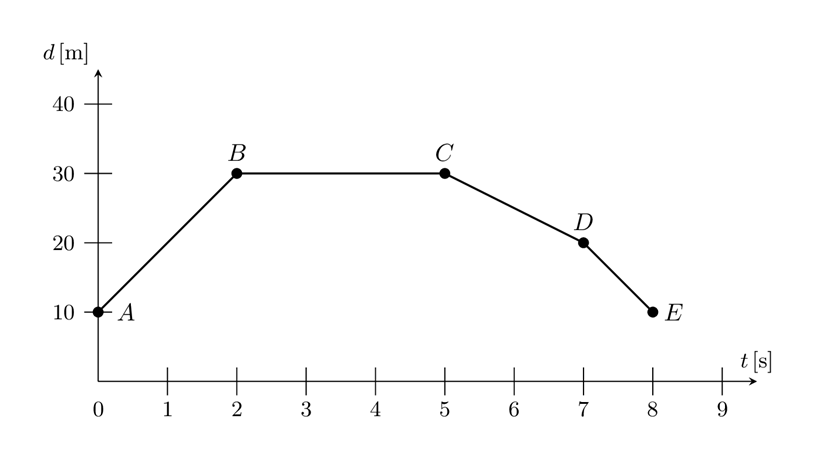
\includegraphics[scale=1.5]{Examen_Grafica_01.png}
    % \end{figure}
    % \question \label{grafica_01} ¿Qué posición tenía el objeto a los cuatro segundos posteriores al inicio de su movimiento?
    % \begin{tasks}(4)
    %     \task \SI{0}{\meter}
    %     \task \SI{10}{\meter}
    %     \task \SI{20}{\meter}
    %     \task \SI{30}{\meter}
    % \end{tasks}
    % \question \label{grafica_02} ¿Cuál es la magnitud de la velocidad del objeto en el intervalo D - E?
    % \begin{tasks}(4)
    %     \task \SI{0}{\meter\per\second}
    %     \task \SI{-5}{\meter\per\second}
    %     \task \SI{-10}{\meter\per\second}
    %     \task \SI{-20}{\meter\per\second}
    % \end{tasks}
    % \question \label{grafica_03} ¿Qué magnitud tiene la velocidad del objeto en el intervalo A -B?
    % \begin{tasks}(4)
    %     \task \SI{0}{\meter\per\second}
    %     \task \SI{10}{\meter\per\second}
    %     \task \SI{15}{\meter\per\second}
    %     \task \SI{50}{\meter\per\second}
    % \end{tasks}
    % \question \label{grafica_04} ¿Cuál fue la posición final del objeto?
    % \begin{tasks}(4)
    %     \task \SI{0}{\meter}
    %     \task \SI{10}{\meter}
    %     \task \SI{20}{\meter}
    %     \task \SI{30}{\meter}
    % \end{tasks}

    \section{(3 puntos) Movimiento uniformemente acelerado.}
    
    \question Si un objeto en movimiento reduce su aceleración, en una gráfica que describe la velocidad del objeto contra tiempo, el valor de la pendiente de la recta que describe el movimiento es:
    \begin{tasks}(4)
        \task Cero
        \task Positiva
        \task Negativa
        \task Alternante
    \end{tasks}
    \question Cuando un objeto en movimiento presenta una aceleración constante, en una gráfica que describe la velocidad del objeto contra tiempo, el valor de la pendiente de la recta que describe el movimiento es:
    \begin{tasks}(4)
        \task Cero
        \task Positiva
        \task Negativa
        \task Alternante
    \end{tasks}
    % \question Considera la siguiente gráfica de velocidad contra tiempo. ¿Cuál es valor de la aceleración del objeto en el intervalo B - C?
    % \begin{figure}[H]
    %     \centering
    %     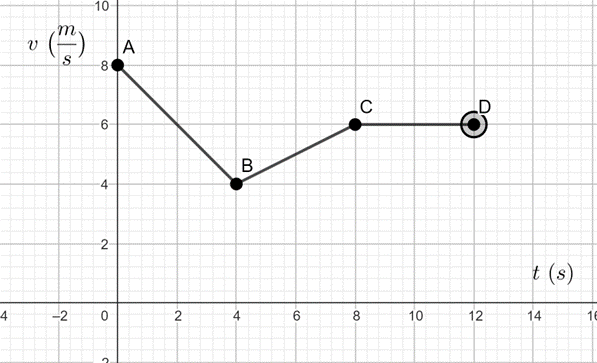
\includegraphics[scale=1.5]{Examen_Grafica_02.png}
    % \end{figure}
    % \begin{tasks}(4)
    %     \task \SI{-1}{\meter\per\square\second}
    %     \task \SI{0}{\meter\per\square\second}
    %     \task \SI{0.5}{\meter\per\square\second}
    %     \task \SI{1}{\meter\per\square\second}
    % \end{tasks}
    % \question \textbf{Problema de ejecución.} Un auto deportivo acelera desde el reposo hasta alcanzar \SI{95}{\kilo\meter\per\hour} en \SI{4.5}{\second}. ¿Cuál es su aceleración?
    % \begin{tasks}(4)
    %     \task \SI{3.11}{\meter\per\square\second}
    %     \task \SI{5.86}{\meter\per\square\second}
    %     \task \SI{22.11}{\meter\per\square\second}
    %     \task \SI{26.38}{\meter\per\square\second}
    % \end{tasks}
    \question \label{Ejercicio_04} \textbf{Ejercicio de ejecución. } Una persona viaja en motocicleta a una velocidad de \SI{3}{\meter\per\second} y acelera constantemente a razón de \SI{0.4}{\meter\per\square\second}. ¿Qué distancia recorrerá después de 1 minuto?
    \begin{tasks}(4)
        \task \SI{900}{\meter}
        \task \SI{1000}{\meter}
        \task \SI{1500}{\meter}
        \task \SI{2000}{\meter}
    \end{tasks}
    
    \section{(2 puntos) Caída libre y tiro vertical.}
    
    % \question Un objeto que experimenta una caída libre, se estudia considerando que el objeto está sujeto a una aceleración de tipo:
    % \begin{tasks}(4)
    %     \task Ascendente.
    %     \task Descendente.
    %     \task Nula.
    %     \task Constante.
    % \end{tasks}
    % \question Revisa el siguiente enunciado \enquote{Una canica se deja caer desde una ventana y tarda \num{5} segundos en llegar al suelo. ¿A qué altura se dejó caer la canica?} 
    % \\[0.3em]
    % ¿Cuál de las siguientes expresiones nos resuelve el problema? \textbf{Nota: } Solo identifica la expresión, no se pide obtener la altura.
    % \begin{tasks}(4)
    %     \task $y = \dfrac{1}{2} \big( v_{i} + v_{f} \big) \, t$
    %     \task $y = v_{i} \, t + \dfrac{1}{2} g \, t^{2}$
    %     \task $2 \, g \, y = v_{f}^{2} - v_{i}^{2}$
    %     \task $v_{f} = v_{i} + g \, t$
    % \end{tasks}
    % \question Completa la siguiente frase: Cuando un objeto es lanzado hacia arriba, alcanza la altura máxima cuando su velocidad final $(v_{f})$ es \rule{2cm}{0.1mm}
    % \begin{tasks}(4)
    %     \task $v_{f} = 2 \, v_{i}$
    %     \task $v_{f} = v_{i}^{2}$
    %     \task $v_{f} = \dfrac{v_{i}}{2}$
    %     \task $v_{f} = 0$
    % \end{tasks}
    % \question El tiempo de vuelo de un objeto en tiro vertical se obtiene con la siguiente expresión:
    % \begin{tasks}(4)
    %     \task $t_{\text{vuelo}} = - \dfrac{2 \, v_{i}}{g}$
    %     \task $t_{\text{vuelo}} = - \dfrac{2 \, v_{f}}{g}$
    %     \task $t_{\text{vuelo}} = - \dfrac{2 \, v_{i}^{2}}{g}$
    %     \task $t_{\text{vuelo}} = - \dfrac{2 \, v_{f}^{2}}{g}$
    % \end{tasks}
    % \question Cuando un objeto se lanza verticalmente hacia arriba, se sabe que conforme se deplaza su velocidad \rule{2cm}{0.1mm}
    % \begin{tasks}(4)
    %     \task Es constante.
    %     \task Es cero.
    %     \task Aumenta.
    %     \task Disminuye.
    % \end{tasks}
    \question \label{Ejercicio_05} \textbf{Ejercicio de ejecución. } En su visita a la Torre Latinoamericana, Tobías dejó caer un muñeco desde el piso \num{44} y tardó \SI{5.81}{\second} en caer al piso (suponiendo que no hubo algún obstáculo durante la caída). Calcula la altura del piso \num{44}.
    \begin{tasks}(4)
        \task \SI{160.21}{\meter}
        \task \SI{165.57}{\meter}
        \task \SI{307.18}{\meter}
        \task \SI{331.14}{\meter}
    \end{tasks}
    \question \label{Ejercicio_06} \textbf{Ejercicio de ejecución. } Se lanza verticalmente hacia arriba una esfera metálica con una velocidad cuya magnitud es de \SI{20}{\meter\per\second}. ¿Qué distancia recorre a los \num{2} segundos?
    \begin{tasks}(4)
        \task \SI{15.09}{\meter}
        \task \SI{20.38}{\meter}
        \task \SI{51.19}{\meter}
        \task \SI{59.62}{\meter}
    \end{tasks}

    \section{(3 puntos) Movimiento circular.}

    \question Es la recta que toca en un solo punto a la circunferencia \rule{2cm}{0.1mm}
    \begin{tasks}(4)
        \task Secante
        \task Tangente
        \task Cuerda
        \task Radio
    \end{tasks}
    \question \label{Ejercicio_07} \textbf{Ejercicio de ejecución. } La turbina de una planta hidroeléctrica gira a razón de 75 rpm. ¿Cuál es el desplazamiento angular en radianes de la punta de una de las hélices de la turbina durante un minuto?
    \begin{tasks}(4)
        \task \SI{150.00}{\radian}
        \task \SI{235.61}{\radian}
        \task \SI{471.23}{\radian}
        \task \SI{785.39}{\radian}
    \end{tasks}
    % \question \label{Ejercicio_08} \textbf{Ejercicio de ejecución. } Un objeto está atado a una cuerda y se mueve en un círculo horizontal de \SI{90}{\centi\meter} de radio. Sin considerar los efectos de la gravedad, el objeto tiene una frecuencia de \num{80} rpm. ¿Cuál es la velocidad lineal que experimenta?
    % \begin{tasks}(4)
    %     \task \SI{7.53}{\meter\per\second}
    %     \task \SI{47.37}{\meter\per\second}
    %     \task \SI{452.38}{\meter\per\second}
    %     \task \SI{753.98}{\meter\per\second}
    % \end{tasks}
    \question \label{Ejercicio_09} \textbf{Ejercicio de ejecución. } Una hélice gira inicialmente con una velocidad angular cuya magnitud es de \SI{10}{\radian\per\second} y recibe una aceleración constante cuya magnitud es de \SI{3}{\radian\per\square\second}. ¿Cuál será la magnitud de su velocidad angular después de \num{7} segundos?
    \begin{tasks}(4)
        \task \SI{30}{\radian\per\second}
        \task \SI{31}{\radian\per\second}
        \task \SI{35}{\radian\per\second}
        \task \SI{36}{\radian\per\second}
    \end{tasks}

    \section{(3 puntos) Leyes de Newton.}

    \question ¿Qué es una fuerza?
    \begin{tasks}
        \task Es la masa de un cuerpo.
        \task Es la suma del peso y la masa.
        \task Es la interacción entre dos cuerpos.
        \task Es la reacción a distancia entre dos cuerpos.
    \end{tasks}
    \question Relaciona las columnas con las letras y los números.
    
    Son las leyes de Newton:
    
    \begin{minipage}[t]{0.4\linewidth}
    \begin{parts}
        \part Primera ley.
        \part Segunda ley.
        \part Tercera ley.
    \end{parts}
    \end{minipage}
    \hspace{-0.5cm}
    \begin{minipage}[t]{0.5\linewidth}
        \begin{enumerate}[label=\arabic*)]
            \itemsep0em
            \item De gravitación universal.
            \item De acción y reacción.
            \item De inercia.
            \item Relación entre masa y aceleración.
        \end{enumerate}
    \end{minipage}
    \begin{tasks}(4)
        \task a-1, \, b-2, \, c-3
        \task a-2, \, b-3, \, c-1
        \task a-3, \, b-4, \, c-2
        \task a-3, \, b-4, \, c-1
    \end{tasks}
    
    % \question ¿Cuál es la masa en la Tierra de un objeto que pesa \SI{490.5}{\newton} (Newtons)?
    % \begin{tasks}(4)
    %     \task \SI{40}{\kilo\gram}
    %     \task \SI{50}{\kilo\gram}
    %     \task \SI{60}{\kilo\gram}
    %     \task \SI{100}{\kilo\gram}
    % \end{tasks}

    % \newpage

    % \question Supongamos que vamos de regreso a casa en un automóvil y se presenta una falla, comenzamos a empujarlo al taller mecánico más cercano. Cuando el automóvil comienza a moverse: ¿Cómo es la fuerza que ejerces sobre el automóvil en comparación con la que éste ejerce sobre ti? 
    % \begin{tasks}
    %     \task La fuerza que ejerce el automóvil es igual en magnitud y opuesta en dirección a la que el automóvil ejerce sobre ti.
    %     \task La fuerza que ejerce el automóvil es mayor en magnitud y en la misma dirección a la que el automóvil ejerce sobre ti.
    %     \task La fuerza que ejerce el automóvil es menor en magnitud y en dirección perpendicular a la que el automóvil ejerce sobre ti.
    %     \task La fuerza que ejerce el automóvil es igual en magnitud y en dirección oblicua a la que el automóvil ejerce sobre ti.
    % \end{tasks}
    % \question \textbf{Ejercicio de ejecución. } Sabemos que la fuerza es una cantidad vectorial, del siguiente vector de fuerza con una magnitud de $\va{F} = \SI{15}{\newton}$ y que tiene una dirección de $\theta = \ang{50}$, ¿cuánto vale la componente $F_{y}$ en la dirección del eje de las ordenadas?
    % \begin{tasks}(4)
    %     \task \SI{9.46}{\newton}
    %     \task \SI{11.49}{\newton}
    %     \task \SI{15.05}{\newton}
    %     \task \SI{17.87}{\newton}
    % \end{tasks}
    % \question \textbf{Ejercicio de ejecución. } Resolviendo en una mesa de fuerzas las componentes de un sistema de vectores, se tiene que las componentes del vector resultante $\va{R}$ son $R_{x} = \SI{10}{\newton}$ y $R_{y} = \SI{8}{\newton}$. ¿Cuál es el ángulo $\theta_{R}$ que se forma con respecto al eje $y$?
    % \begin{tasks}(4)
    %     \task $\theta_{R} = \ang{38.65}$
    %     \task $\theta_{R} = \ang{51.34}$
    %     \task $\theta_{R} = \ang{60.38}$
    %     \task $\theta_{R} = \ang{90}$
    % \end{tasks}
    \question \label{Ejercicio_10} \textbf{Ejercicio de ejecución. } Calcula la masa de una caja en kilogramos, si al recibir una fuerza cuya magnitud es de \SI{300}{\newton} le produce una aceleración con una magnitud de \SI{150}{\centi\meter\per\square\second}.
    \begin{tasks}(4)
        \task \SI{2}{\kilo\gram}
        \task \SI{10}{\kilo\gram}
        \task \SI{100}{\kilo\gram}
        \task \SI{200}{\kilo\gram}
    \end{tasks}
    % \question \textbf{Ejercicio de ejecución. } Calcula la magnitud de la fuerza que se le aplica a un sillón de \SI{10}{\kilo\gram} de masa si adquiere una aceleración cuya magnitud es de \SI{2.5}{\meter\per\square\second}.
    % \begin{tasks}(4)
    %     \task \SI{5}{\newton}
    %     \task \SI{25}{\newton}
    %     \task \SI{50}{\newton}
    %     \task \SI{75}{\newton}
    % \end{tasks}

    \section{(2 puntos) Ley de gravitación universal.}

    % \question \textbf{Problema de ejecución. } Calcula la distancia a la que se deben de colocar dos masas iguales de \SI{100}{\kilo\gram} para que se atraigan con una fuerza gravitacional de \SI{100}{\newton}.
    % \begin{tasks}(4)
    %     \task $\SI{8.16d-5}{\meter}$
    %     \task $\SI{9.81d-5}{\meter}$
    %     \task $\SI{6.67d-9}{\meter}$
    %     \task $\SI{6.67d-11}{\meter}$
    % \end{tasks}
    \question En acuerdo con la ley de gravitación universal cuando dos objetos se acercan, la fuerza de atracción gravitacional entre ellos: \rule{2cm}{0.1mm}
    \begin{tasks}(4)
        \task Disminuye
        \task Aumenta
        \task Es constante
        \task Se anula
    \end{tasks}
    \question \label{Ejercicio_11} \textbf{Ejercicio de ejecución. } Una barra metálica cuyo peso tiene una magnitud de \SI{800}{\newton} se acerca a otra de \SI{1200}{\newton} hasta que la distancia entre sus centros es de \SI{80}{\centi\meter}. ¿Con qué magnitud de fuerza gravitacional se atraen?
    \begin{tasks}(4)
        \task \SI{1.039d-5}{\newton}
        \task \SI{1.039d-6}{\newton}
        \task \SI{8.317d-7}{\newton}
        \task \SI{1.000d-8}{\newton}
    \end{tasks}

    \newpage

    \section{(3 puntos) Satélites.}

    \question Planeta del Sistema Solar que no tiene satélites naturales: \rule{2cm}{0.1mm}
    \begin{tasks}(4)
        \task Marte
        \task Mercurio
        \task Júpiter
        \task Neptuno
    \end{tasks}
    % \question Es el nombre del primer satélite artificial que orbitó la Tierra: \rule{2cm}{0.1mm}
    % \begin{tasks}(4)
    %     \task Soyuz
    %     \task Sputnik
    %     \task Mir
    %     \task Korolev
    % \end{tasks}
    \question El 17 de junio de 1985 fue lanzado al espacio desde Cabo Cañaveral, Florida, el primer satélite de comunicaciones mexicano, fue nombrado como: \rule{2cm}{0.1mm}
    \begin{tasks}(4)
        \task Satmex 5
        \task Solidaridad I
        \task Morelos I
        \task Hidalgo I
    \end{tasks}
    \question La velocidad \rule{2cm}{0.1mm}, es la velocidad necesaria para que un objeto supere la atracción gravitatoria y no vuelva a caer a la superficie de un cuerpo celeste.
    \begin{tasks}(4)
        \task Angular
        \task Tangencial
        \task De escape
        \task Lineal
    \end{tasks}


    \section{(3 puntos) Leyes de Kepler y el Sistema Solar.}

    % \question De la primera ley de Kepler ¿cuál es el espacio geométrico que explica la trayectoria de un planeta?
    % \begin{tasks}(4)
    %     \task Círculo.
    %     \task Parábola.
    %     \task Elipse.
    %     \task Hipérbola.
    % \end{tasks}
    \question De la primera ley de Kepler, el Sol se encuentra en un punto de la elipse, ¿cuál es ese punto?
    \begin{tasks}(4)
        \task Centro.
        \task Vértice.
        \task Eje mayor.
        \task Foco.
    \end{tasks}
    \question El punto de la órbita de un planeta en donde se encuentra más cerca del Sol se llama: \rule{2cm}{0.1mm}
    \begin{tasks}(4)
        \task Afelio
        \task Perihelio
        \task Periodo
        \task Hemiciclo
    \end{tasks}
    \question \rule{2cm}{0.1mm} es el sexto planeta del Sistema Solar considerando su posición a partir del Sol.
    \begin{tasks}(4)
        \task Marte.
        \task Saturno.
        \task Júpiter.
        \task Neptuno.
    \end{tasks}
   
    \section{(3 puntos) Plantas generadoras de electricidad y su transmisión.}

    % \question Por experiencia sabemos que los materiales tienen un equilibrio en su carga eléctrica, es decir, son eléctricamente \rule{2cm}{0.1mm}.
    % \begin{tasks}(4)
    %     \task Positivos.
    %     \task Neutros.
    %     \task Negativos.
    %     \task Aislantes.
    % \end{tasks}
    % \question Es la fuerza impulsora que permite el flujo de carga eléctrica a través de un conductor:
    % \begin{tasks}(4)
    %     \task Resistencia.
    %     \task Corriente.
    %     \task Voltaje.
    %     \task Conductividad.
    % \end{tasks}
    % \question \textbf{Ejercicio de ejecución. } Cierto foco tiene una resistencia de \SI{240}{\ohm} cuando se enciende. ¿Cuánta corriente fluirá a través del foco cuando se conecta a \SI{120}{\volt}? que es su voltaje de operación normal.
    % \begin{tasks}(4)
    %     \task \SI{0.5}{\ampere}
    %     \task \SI{1.0}{\ampere}
    %     \task \SI{1.5}{\ampere}
    %     \task \SI{2.0}{\ampere}
    % \end{tasks}
    % \question\textbf{Ejercicio de ejecución. } Un calentador eléctrico utiliza \SI{5.0}{\ampere} cuando se conecta a \SI{110}{\volt}. Determina su resistencia.
    % \begin{tasks}(4)
    %     \task \SI{12}{\ohm}
    %     \task \SI{22}{\ohm}
    %     \task \SI{52}{\ohm}
    %     \task \SI{72}{\ohm}
    % \end{tasks}
    % \question \textbf{Ejercicio de ejecución. } ¿Cuál es el voltaje a través de una parrilla eléctrica que consume \SI{5.0}{\ampere} cuando su resistencia caliente es de \SI{24}{\ohm}?
    % \begin{tasks}(4)
    %     \task \SI{100}{\volt}
    %     \task \SI{110}{\volt}
    %     \task \SI{120}{\volt}
    %     \task \SI{220}{\volt}
    % \end{tasks}

    \question Son aquellas plantas que generan electricidad por medio de vapor conducido a una turbina que se conecta a un generador:
    \begin{multicols}{2}
    \begin{tasks}
        \task Nuclear, geotérmica, térmica.
        \task Eólica, geotérmica, biomasa.
        \task Hidroeléctrica, nuclear, geotérmica.
        \task Térmica, solar, geotérmica.
    \end{tasks}
    \end{multicols}

    % \question Nombre del científico a quien se le asocia el principio de inducción por el cual la energía mecánica en una turbina, se transforma en el generador en energía eléctrica.
    % \begin{tasks}(4)
    %     \task Raleigh.
    %     \task Fermat.
    %     \task Faraday.
    %     \task Ampere.
    % \end{tasks}
    \question En una planta nuclear, el proceso mediante el cual se va dividiendo al átomo del combustible se llama: \rule{2cm}{0.1mm} nuclear, en donde se libera la energía que permite calentar el agua para convertirla en vapor y mover las turbinas.
    \begin{tasks}(4)
        \task Fisión
        \task Fusión
        \task Enriquecimiento
        \task Colapso
    \end{tasks}

    \newpage

    \question La capacidad de transmisión de energía eléctrica de una línea se determina por \rule{2cm}{0.1mm} de los conductores y \rule{2cm}{0.1mm} entre las torres.
    \begin{multicols}{2}
    \begin{tasks}
        \task la capacidad de carga - la distancia.
        \task el diámetro - la altura.
        \task el material - la red.
        \task la densidad - la forma.
    \end{tasks}
    \end{multicols}

    \section{(2 puntos) Ley de inducción de Faraday.}

    \question La ley de inducción de Faraday establece que la variación \rule{2cm}{0.1mm} en una bobina del rotor del generador, induce \rule{2cm}{0.1mm} en una bobina del estator.
    \begin{tasks}
        \task del flujo eléctrico - una intensidad magnética.
        \task del flujo magnético - una corriente eléctrica.
        \task del flujo cinético - una corriente eléctrica.
        \task de la energía potencial - una corriente eléctrica.
    \end{tasks}
    \question Se le llama \rule{2cm}{0.1mm} al proceso en el generador, en el cual se modifica la corriente eléctrica alterna a una corriente eléctrica directa.
    \begin{tasks}(4)
        \task Rectificación
        \task Amplificación
        \task Reducción
        \task Nulificación
    \end{tasks}

    \section{(6 puntos) Calor, Trabajo y Energía.}
    
    \question Es la capacidad de un sistema físico para realizar un trabajo:
    \begin{tasks}(4)
        \task Potencia.
        \task Fuerza.
        \task Energía.
        \task Movimiento.
    \end{tasks}
    % \question En un problema se nos proporciona el valor de energía cinética $(E_{k})$ así como la masa $(m)$ de un objeto, se nos pide obtener la velocidad $(v)$ con la que se desplaza el objeto, ¿qué expresión de las siguientes es la que debemos de utilizar?
    % \begin{tasks}(4)
    %     \task $v = \sqrt{\dfrac{E_{k} \, m}{2}}$
    %     \task $v = \sqrt{\dfrac{E_{k}}{2 \, m}}$
    %     \task $v = \sqrt{\dfrac{2 \, m}{E_{k}}}$
    %     \task $v = \sqrt{\dfrac{2 \, E_{k}}{m}}$
    % \end{tasks}
    \question La energía total (energía mecánica) de un sistema es:
    \begin{tasks}
        \task La suma de la energía potencial y la energía cinética.
        \task La suma de la energía potencial y la energía eléctrica.
        \task La diferencia de la energía potencial y la energía cinética.
        \task El producto de la energía potencial y la energía térmica.
    \end{tasks}
    \question \rule{2cm}{0.1mm} es una forma de energía que se transfiere entre dos sistemas (o entre partes de un sistema) debido a \rule{2cm}{0.1mm}.
    \begin{tasks}
        \task El calor - una diferencia de temperatura.
        \task La energía cinética - al incremento de calor.
        \task El calor - una suma de temperatura.
        \task La energía cinética - a un descenso de temperatura.
    \end{tasks}
    % \question \textbf{Ejercicio de ejecución. } Se realiza un trabajo mecánico de \SI{3500}{\joule} para elevar una cubeta con arena cuyo peso tiene una magnitud de \SI{350}{\newton}. Determina la altura a la que se elevó la cubeta.
    % \begin{tasks}(4)
    %     \task \SI{5}{\meter}
    %     \task \SI{10}{\meter}
    %     \task \SI{15}{\meter}
    %     \task \SI{20}{\meter}
    % \end{tasks}
    
    % \question \textbf{Ejercicio de ejecución. } ¿En qué piso de un estacionamiento se encuentra un auto de \SI{840}{\kilo\gram} para que su energía potencial sea de \SI{39600}{\joule}? Cada piso mide \SI{2.4}{\meter}.
    % \begin{tasks}(4)
    %     \task Planta baja.
    %     \task Piso 1.
    %     \task Piso 2.
    %     \task Piso 3.
    % \end{tasks}

    \question En la siguiente figura se presentan los mecanismos de transferencia de calor, identifica cada letra de la figura con el inciso correspondiente de cada mecanismo.
    \begin{figure}[H]
        \centering
        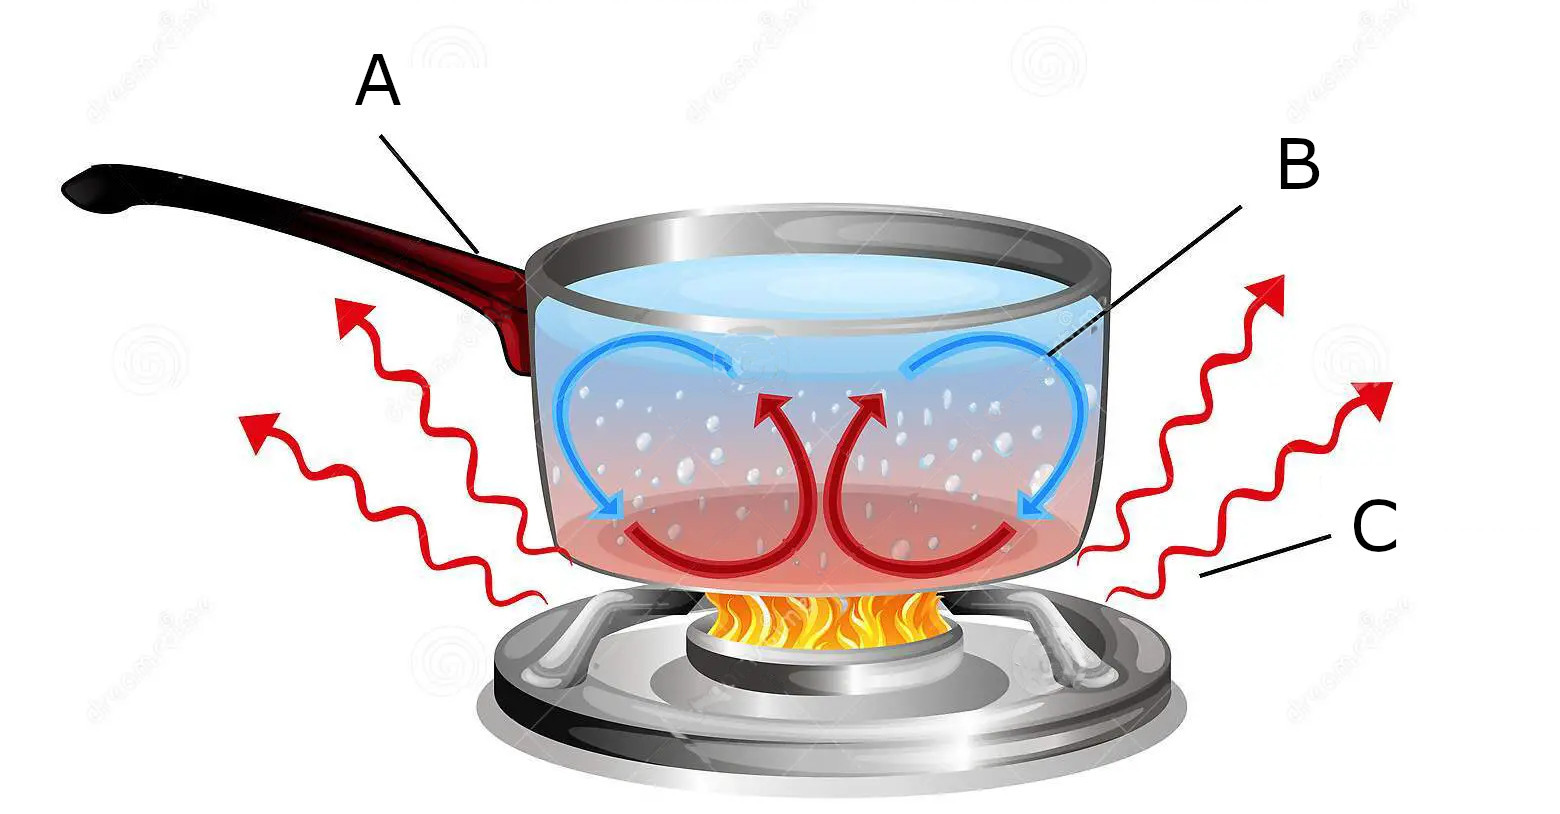
\includegraphics[scale=0.2]{Transferencia_Calor_01.jpg}
    \end{figure}
    \begin{multicols}{4}
    \begin{enumerate}[label=\Roman*)]
        \item Convección.
        \item Radiación.
        \item Conducción.
        \item Evaporación.
    \end{enumerate}
    \end{multicols}
    \begin{tasks}
        \task A - I, B - II, C - III
        \task A - IV, B - I, C - II
        \task A - II, B - III, C - I
        \task A - III, B - I, C - II
    \end{tasks}
    % \question \textbf{Ejercicio de ejecución. } El flúor es un elemento químico que está en el grupo de los halógenos. Su punto de ebullición de encuentra en los \SI{85.03}{\kelvin}. ¿Cuánto equivale esa temperatura en grados Celsius?
    % \begin{tasks}(4)
    %     \task \SI{-188.12}{\degreeCelsius}
    %     \task \SI{-456.15}{\degreeCelsius}
    %     \task \SI{30.15}{\degreeCelsius}
    %     \task \SI{-600.15}{\degreeCelsius}
    % \end{tasks}

    \question \label{Ejercicio_12} \textbf{Ejercicio de ejecución. } Calcula la magnitud de la velocidad de una caja cuya masa es de \SI{4}{\kilo\gram} y tiene una energía cinética de \SI{100}{\joule}.
    \begin{tasks}(4)
        \task \SI{4.07}{\meter\per\second}
        \task \SI{5.07}{\meter\per\second}
        \task \SI{6.07}{\meter\per\second}
        \task \SI{7.07}{\meter\per\second}
    \end{tasks}
    \question \label{Ejercicio_13} \textbf{Ejercicio de ejecución. } La novela de ciencia ficción \textit{Fahrenheit 451} del escritor Rad Bradbury, el título hace referencia a la temperatura en la que el papel de los libros se inflama. ¿Cuánto equivale esa temperatura $(451 ^{\circ}\text{F})$ en grados Celsius?
    \begin{tasks}(4)
        \task \SI{200.46}{\degreeCelsius}
        \task \SI{232.77}{\degreeCelsius}
        \task \SI{350.63}{\degreeCelsius}
        \task \SI{500.45}{\degreeCelsius}
    \end{tasks}
    % \question \label{Ejercicio_14} \textbf{Ejercicio de ejecución. } A una temperatura de \SI{15}{\degreeCelsius} una varilla de hierro tiene una longitud de \SI{5}{\meter}. ¿Cuál será la longitud de la varilla al aumentar la temperatura a \SI{25}{\degreeCelsius}? El valor de $\alpha_{Fe}$ está en el Formulario.
    % \begin{tasks}(4)
    %     \task \SI{5.8775}{\meter}
    %     \task \SI{5.08775}{\meter}
    %     \task \SI{5.008775}{\meter}
    %     \task \SI{5.0008775}{\meter}
    % \end{tasks}

    \section{(2 puntos) Máquinas y eficiencia.}

    % \question La eficiencia $(\eta)$ de una máquina ideal es:
    % \begin{tasks}(4)
    %     \task $\eta < 100 \%$
    %     \task $\eta > 100 \%$
    %     \task $\eta = 0 \%$
    %     \task $\eta = 100 \%$
    % \end{tasks}
    
    \question Las máquinas reales experimentan pérdidas de energía, que en conformidad con la ley de conservación de energía, esa pérdida \rule{2cm}{0.1mm}
    \begin{multicols}{2}
    \begin{tasks}
        \task se transforma en electricidad.
        \task aumenta su energía potencial.
        \task se disipa en forma de calor.
        \task incrementa su velocidad angular.
    \end{tasks}
    \end{multicols}
    \question \label{Ejercicio_15} \textbf{Ejercicio de ejecución. } Una celda solar que está en desarrollo, transforma energía solar a energía eléctrica, si se sabe que se le suministran \SI{748}{\joule} y a la salida devuelve \SI{500}{\joule}, calcula la eficiencia en porcentaje de la celda solar.
    \begin{tasks}(4)
        \task $\eta = 50.15 \%$
        \task $\eta = 66.84 \%$
        \task $\eta = 72.03 \%$
        \task $\eta = 100.00 \%$
    \end{tasks}
    
    \section{(2 puntos) Piezoelectricidad.}

    \question La piezoelectricidad es un fenómeno físico en el cual ciertos materiales tienen la capacidad de generar una \rule{2cm}{0.1mm} eléctrica.
    \begin{tasks}(4)
        \task Resistencia
        \task Carga
        \task Conductividad
        \task Potencia
    \end{tasks}
    \question Son materiales que presentan el efecto piezoeléctrico:
    \begin{multicols}{2}
    \begin{tasks}
        \task Cristales, Materia orgánica, Gases.
        \task Cristales, Líquidos, Cerámicos.
        \task Cristales, Cerámicos, Polímeros.
        \task Plásticos, Cerámicos, Polímeros.
    \end{tasks}
    \end{multicols}

    \section{(2 puntos) Superconductividad.}

    \question Un material superconductor se caracteriza por que su resistencia interna \rule{2cm}{0.1mm}
    \begin{tasks}(4)
        \task Se incrementa.
        \task Vale cero.
        \task Se hace negativa.
        \task No cambia.
    \end{tasks}
    \question El valor de temperatura en el que se presenta el estado superconductor en un material, se le conoce como \rule{2cm}{0.1mm}
    \begin{multicols}{2}
    \begin{tasks}
        \task Temperatura crítica.
        \task Temperatura mínima.
        \task Temperatura máxima.
        \task Temperatura estándar.
    \end{tasks}
    \end{multicols}

    \section{(2 puntos) Sustentabilidad y contaminación.}

    \question La inversión térmica es un fenómeno que se presenta cuando la temperatura del aire \rule{2cm}{0.1mm} conforme subimos en altura.
    \begin{tasks}(4)
        \task Disminuye
        \task Aumenta
        \task No cambia
        \task Se equilibra
    \end{tasks}
    \question Las partículas PM10 son aquellas partículas sólidas o líquidas de diferente composición y tamaño que se encuentran dispersas en la atmósfera y que tienen un diámetro \rule{2cm}{0.1mm}
    \begin{tasks}(4)
        \task Mayor que \SI{10}{\micro\meter}
        \task Menor que \SI{10}{\micro\meter}
        \task Igual a \SI{0.1}{\micro\meter}
        \task Igual a \SI{0.01}{\micro\meter}
    \end{tasks}

\end{questions}

    \newpage

\textbf{\huge{Formulario.}}
\begin{table}[H]
    \centering
    \setlength{\tabcolsep}{40pt}
    \renewcommand{\arraystretch}{2}
    \begin{tabular}{c  c}
        \multicolumn{2}{c}{Cantidades} \\
            $g = \SI{9.81}{\meter\per\square\second}$ & $\SI{1}{\kilo\meter} = \SI{1000}{\meter}$  \\
            $\SI{1}{\hour} = \SI{3600}{\second}$ & $1$ milla = \SI{1.609}{\kilo\meter} \\ \hline
        \multicolumn{2}{c}{Movimiento rectilíneo uniforme} \\
            $v = \dfrac{d}{t}$ & $v = \dfrac{x_{f} - x_{i}}{t_{f} - t_{i}}$ \\ \hline
		\multicolumn{2}{c}{Movimiento uniformemente acelerado} \\
            $a = \dfrac{v_{f} - v_{i}}{t_{f} - t_{i}}$ & \\
            $v_{f} = v_{i} + a \, t$ & $d = \dfrac{1}{2} \big( v_{i} + v_{f} \big) \, t$ \\
            $d = v_{i} \, t + \dfrac{1}{2} a \, t^{2}$ & $2 \, a \, d = v_{f}^{2} - v_{i}^{2}$ \\ \hline
        \multicolumn{2}{c}{Caída libre y Tiro vertical} \\
            $v_{f} = v_{i} + g \, t$ & $y = \dfrac{1}{2} \big( v_{i} + v_{f} \big) \, t$ \\
            $y = v_{i} \, t + \dfrac{1}{2} g \, t^{2}$ & $2 \, g \, y = v_{f}^{2} - v_{i}^{2}$ \\ 
            $y_{\text{máx}} = - \dfrac{v_{i}^{2}}{2 \, g}$ & $t_{\text{subida}} = - \dfrac{v_{i}}{g}$ \\ \hline
            % \multicolumn{2}{c}{Vectores} \\
            % $\abs{\va{R}} = \sqrt{R_{x}^{2} + R_{y}^{2}}$ & $\theta_{R} = \tan^{-1} \left( \dfrac{R_{y}}{R_{x}} \right)$ \\
            % $R_{x} = \cos \theta \cdot \abs{\va{R}}$ & $R_{x} = \text{sen} \, \theta \cdot \abs{\va{R}}$ \\ \hline
        \multicolumn{2}{c}{Movimiento circular} \\
        \ang{360} = $2 \, \pi$ radianes & $T = \dfrac{\text{segundos transcurridos}}{\text{1 ciclo}}$ \\
        $f = \dfrac{\text{número de ciclos}}{\text{1 segundo}}$ & $\omega = \dfrac{\theta}{t}$ \\
        $\omega = \dfrac{\theta_{f} - \theta_{i}}{t_{f} - t_{i}}$ & $\omega = \dfrac{2 \, \pi \, \text{rad}}{T}$ \\
        $\omega = 2 \, \pi \, f $ & $\omega_{m} = \dfrac{\omega_{f} + \omega_{i}}{2}$ \\
        $v_{L} = \dfrac{2 \, \pi \, r}{T}$ & $v_{L} = \omega \cdot r$ \\
    \end{tabular}
\end{table}
\begin{table}[H]
    \centering
    \setlength{\tabcolsep}{40pt}
    \renewcommand{\arraystretch}{2.5}
    \begin{tabular}{c  c}
        \multicolumn{2}{c}{Movimiento circular} \\
            $\alpha = \dfrac{\omega_{f} - \omega_{i}}{t_{f} - t_{i}}$ & $a_{c} = \dfrac{v^{2}}{r}$ \\
            $\theta = \dfrac{\omega_{f}^{2} - \omega_{i}^{2}}{2 \, \alpha}$ & $\theta = \omega_{i} \, t + \dfrac{\alpha \, t^{2}}{2}$ \\
            $\theta = \dfrac{\alpha \, t^{2}}{2}$ & $\theta = \dfrac{\omega_{f} + \omega_{i}}{2} \, t$ \\
            $\theta = \dfrac{\omega_{f}}{2} \, t$ & $\theta = \dfrac{\omega_{f}^{2}}{2 \, \alpha}$ \\
            $\omega_{f} = \omega_{i}^{2} + 2 \, \alpha \, \theta$ & $\omega_{f} = \omega_{i} + \alpha \, t$ \\
            $\omega_{f} = 2 \, \alpha \, \theta$ & $\omega_{f} = \alpha \, t$ \\ \hline
        \multicolumn{2}{c}{Leyes de Newton y ley de gravitación universal} \\
            $F = m \cdot a$ & $F = G \, \dfrac{m_{1} \cdot m_{2}}{r^{2}}$ \\
            $W = m \, g$ & $G = \displaystyle \SI[per-mode=fraction]{6.67d-11}{\newton\square\meter\per\square\kilo\gram}$ \\ \hline
        % \multicolumn{2}{c}{Electricidad} \\
            % $q = n \cdot e$ & $e = \SI{1.6d-19}{\coulomb}$ \\
            % $V = I \cdot R$ & \\ \hline
        \multicolumn{2}{c}{Calor, trabajo y energía} \\
            $T = F \cdot d$ &  \\
            $E_{k} = \dfrac{1}{2} \, m \, v^{2}$ & $E_{p} = m \, g \, h$ \\
            $\unit{\degreeCelsius} = \dfrac{5}{9} \left( ^{\circ}\text{F} - 32 \right)$ & $^{\circ}\text{F} = \dfrac{9}{5} \, \unit{\degreeCelsius} + 32$ \\
            $K = \unit{\degreeCelsius} + 273.15$ & $\unit{\degreeCelsius} = K - 273.15$ \\
            % $R = \, ^{\circ}\text{F} + 460$ & $\Delta L = \alpha \, L_{i} \, \Delta T$ \\
            $R = \, ^{\circ}\text{F} + 460$ &  \\ \hline
            %  & $\alpha_{Fe} = \SI{11.7d-6}{\degreeCelsius}^{-1}$ \\ \hline
        \multicolumn{2}{c}{Máquinas y eficiencia} \\
            $\eta = \dfrac{W_{s}}{W_{e}} \times 100 \%$ & \\
\end{tabular}
\end{table}

\newpage

En este espacio deberás de incluir el desarrollo completo de los Problemas de Ejecución. El problema se califica de la siguiente manera: \textbf{a) Datos: 0.25 puntos}, \textbf{b) Expresión(es): 0.25 puntos}, \textbf{c) Sustitución: 0.25 puntos} y \textbf{d) Manejo de unidades: 0.25 puntos}.

\vspace*{0.5cm}

Solución al Problema de Ejecución \ref{Ejercicio_01}:

\vspace*{3.5cm}
\rule{0.9\textwidth}{0.3mm}

Solución al Problema de Ejecución \ref{Ejercicio_02}:

\vspace*{3.5cm}
\rule{0.9\textwidth}{0.3mm}

% Solución al Problema de Ejecución \ref{Ejercicio_03}:

% \vspace*{3.5cm}
% \rule{0.9\textwidth}{0.3mm}

Solución al Problema de Ejecución \ref{Ejercicio_04}:

\vspace*{3.5cm}
\rule{0.9\textwidth}{0.3mm}

% \newpage

% \rule{0.9\textwidth}{0.3mm}

Solución al Problema de Ejecución \ref{Ejercicio_05}: 

\vspace*{3.5cm}
\rule{0.9\textwidth}{0.3mm}

\newpage

Solución al Problema de Ejecución \ref{Ejercicio_06}:

\vspace*{3.5cm}
\rule{0.9\textwidth}{0.3mm}

Solución al Problema de Ejecución \ref{Ejercicio_07}:

\vspace*{3.5cm}
\rule{0.9\textwidth}{0.3mm}

% Solución al Problema de Ejecución \ref{Ejercicio_08}:

% \vspace*{3.5cm}
% \rule{0.9\textwidth}{0.3mm}

Solución al Problema de Ejecución \ref{Ejercicio_09}:

\vspace*{3.5cm}
\rule{0.9\textwidth}{0.3mm}

Solución al Problema de Ejecución \ref{Ejercicio_10}:

\vspace*{3.5cm}
\rule{0.9\textwidth}{0.3mm}

Solución al Problema de Ejecución \ref{Ejercicio_11}:

\vspace*{3.5cm}
\rule{0.9\textwidth}{0.3mm}

Solución al Problema de Ejecución \ref{Ejercicio_12}:

\vspace*{3.5cm}
\rule{0.9\textwidth}{0.3mm}

Solución al Problema de Ejecución \ref{Ejercicio_13}:

\vspace*{3.5cm}
\rule{0.9\textwidth}{0.3mm}

% Solución al Problema de Ejecución \ref{Ejercicio_14}:

% \newpage

% \rule{0.9\textwidth}{0.3mm}

Solución al Problema de Ejecución \ref{Ejercicio_15}:

\end{document}